\documentclass[10pt]{article}
\usepackage[compact,small]{titlesec} % makes compact or small section headers
\usepackage[comma,authoryear]{natbib}
\usepackage{graphicx}
\usepackage{amssymb,amsmath}
\usepackage{latexsym}
\usepackage{color}
\usepackage{algorithm}
\usepackage{algpseudocode}
\usepackage{caption}

\usepackage{xspace}
% Silly colors
\definecolor{scarlet}{RGB}{190, 1, 25}
\definecolor{crimson}{RGB}{153, 0, 0}
\definecolor{waterblue}{RGB}{55, 120, 191}
\definecolor{tangerine}{RGB}{249, 115, 6}
\definecolor{grassgreen}{RGB}{77, 164, 9}


% Environments, etc.

\newcommand{\beq}{\begin{equation}}
\newcommand{\eeq}{\end{equation}}
\newcommand{\beqa}{\begin{eqnarray}}
\newcommand{\eeqa}{\end{eqnarray}}
\newcommand{\beqas}{\begin{eqnarray*}}
\newcommand{\eeqas}{\end{eqnarray*}}
\newcommand{\bit}{\begin{itemize}}
\newcommand{\eit}{\end{itemize}}
\newcommand{\benum}{\begin{enumerate}}
\newcommand{\eenum}{\end{enumerate}}

\newcommand{\mmp}[1]{\textcolor{blue}{{\em #1}}}
\newcommand{\formmp}[1]{\textcolor{crimson}{{ #1}}}  %This is text for my personal notes, conjectures, but not ready for distribution
\newcommand{\comment}[1]{}

\newcommand{\topt}{top-$t$\xspace}
\newcommand{\gmms}{\ensuremath{GMM^s}}


\newcommand{\algsamgmm}{\mbox{\sc Sample-from-GMMs}\xspace}
\newcommand{\algrobme}{\mbox{\sc Robust-Mean}\xspace}
\newcommand{\algrobsd}{\mbox{\sc Robust-StDev}\xspace}

% Math mode commands

\newcommand{\sigzero}{\sigma_0}
\newcommand{\pizero}{\pi_0}


\newcommand{\X}{{\mathcal X}}
\newcommand{\ssss}{{\mathbb S}}
\newcommand{\probb}{{\mathbb P}}
\newcommand{\nnnn}{{\mathbb N}}
\newcommand{\idperm}{{\rm id}}


\newcommand{\trace}{\operatorname{trace}}
\newcommand{\geom}{\operatorname{Geo}}
\newcommand{\rank}{\operatorname{rank}}

\newcommand{\ceil}{\operatorname{ceil}}


\newcommand{\G}{{\mathcal G}}
\newcommand{\V}{{\mathcal V}}
\newcommand{\E}{{\mathcal E}}
\newcommand{\EE}{\vec{\mathcal E}}
\newcommand{\T}{{\mathcal T}}
\newcommand{\LL}{{\mathcal L}}
\newcommand{\U}{{\mathcal D}}

\newcommand{\vn}{{\mathbf n}}
\newcommand{\vc}{{\mathbf c}}
\newcommand{\vx}{{\mathbf X}}
\newcommand{\vxt}{{\mathbf X}^{(t)}}
\newcommand{\vxtt}{{\mathbf X}^{()}}

\newcommand{\thetahat}{\hat{\theta}}
\newcommand{\tilthe}{\tilde{\theta}}

\newcommand{\mmax}{_{\rm max}}


\newcommand{\bbone}[1]{{1}_{[#1]}}
\newcommand{\rrr}{{\mathbb R}}
\newcommand{\bigOO}{{\cal O}}
\newcommand{\nchoosek}[2]{C^{#2}_{#1}}  % for now, until i figure out
				        % how to make it look better

\newcommand {\argmax}[2]{\mbox{\raisebox{-1.7ex}{$\stackrel{\textstyle
{\rm #1}}{\scriptstyle #2}$}}\,}
\newcommand{\fracpartial}[2]{\frac{\partial {#1}}{\partial {#2}}}

\newcommand{\inv}{\operatorname{inv}}
\newcommand{\tilpi}{\tilde{\pi}}


% Lengths and formatting

\setlength{\oddsidemargin}{0in}
\setlength{\evensidemargin}{0in}
\setlength{\topmargin}{-1.5cm}
\setlength{\textheight}{9in}
\setlength{\textwidth}{6.5in}
\setlength{\parskip}{.1 em}
%\setlength{\parindent}{0em}
\setlength{\itemsep}{0em}
\setlength{\tabcolsep}{0em}

% Run in section headings to save space
\titleformat{\section}[block]
  {\large\bfseries\filright}
  {\thesection}{6pt}{}
\titlespacing{\section}
  {\parindent}{*2}{\wordsep}

\titleformat{\subsection}[block]
%\titleformat{\subsection}[runin]
  {\normalfont\bfseries}
  {\thesubsection}{6pt}{}
\titlespacing{\subsection}
  {\parindent}{*2}{\wordsep}

\titleformat{\subsubsection}[runin]
  {\normalfont\bfseries}
  {\thesubsubsection}{6pt}{}


\newtheorem{prop}{Proposition}
\newtheorem{remark}[prop]{Remark}

\newlength{\picwi}
\newlength{\tttwi}
\setlength{\tttwi}{\textwidth}

\title{NSASAG Problem 23-02 Comparing ranked lists\\When blocks of items are preserved}
\author{Marina Meil\u{a}\\{\tt mmp@stat.washington.edu}}


\date{October 20, 2023}

\begin{document}

\maketitle

\section{Problem}
\label{sec:problem}
This report follows from a discussion at the NSASAG virtual visit, where this problem came up.

It is common with recommender systems that, for small variations in the ranking algorithm, large variations in the rankings appear, which are due to blocks of items moving together up or down the ranking. For example, assume $B\subset \X$ is a set of $K$ items, which appears in a list  $\pi$ starting at rank $b$. After a small algorithm change, the recommender system outputs the list $\pi'$, where the same block $B$, in approximately the same order, appear at rank $b'$ which can be $\ll b$ or $\gg b$. This would be a very large change between $\pi$ and $\pi'$ in any classical model, but if we assume that the items in block $B$ move ``dependently'', together, then it's not a large change anymore. Note that there could be other blocks $B'$ whose elements also move together up or down ranks. 

In this report I present a simple heuristic to detect such blocks. 


\section{Notation}
\label{sec:notation}
\mmp{The common notation is the same as in {\tt 23-02-mmp.pdf}.}

Let $\pi=(x_1,\ldots x_n)$, $\pi'=(y_1,\ldots y_m)$ be the two lists; we will call lists like these \topt permutations; here $t=n$, respectively $m$. We may denote alternatively $x_j\equiv \pi_j, y_j\equiv \pi'_j$, and $|\pi|=n,|\pi'|=m$; then $\pi_{1:k}\equiv x_{1:k}$ is a prefix of $\pi$. If necessary, we assume $n\geq m$. 

We will assume that the lists $\pi,\pi'$ are drawn from the same probability
distribution $\probb$ over a very large set of items $\X$. The modal
 (most probable, ``true'') permutation of $\probb$ is
denoted by $\sigma_0$. In general, we denote by $\sigma\in \ssss_{\X}$
complete permutations of the elements of $\X$; we also denote with $\sigma$ complete or truncated ``model parameters'', while with $\pi$ we denote observations (always truncated). We will never have access to the entire $\X,\sigzero$ or $\probb$, but we will assume these exist and do math with them. In fact, in some cases, we can assume $\X$ is countable. In general, it will be unreasonable to obtain results that depend strongly on $|\X|$.  In this report, ranking, list, are used interchangeably; for permutations of the entire set $\X$ we may also use the term permutation.

Note that some of the remarks below will not be needed for this problem, as we will only consider the set of items observed in both rankings $\X_0=\pi\cap \pi'|$.


\section{Approach -- Inversion matrices}
\label{sec:Q}
The {\em inversion matrix} $Q(\pi|\pizero)$ is a way to encode the differences of two permutations without loss of information. All distance measures between permutations can be obtained from $Q$.

Here we assume complete permutations $\pi,\pizero$ over a {\em finite} set $\X_0\subset \X$. Then, the inversion matrix $Q(\pi|\pizero)$ is a matrix whose rows and columns are sorted by $\pizero$. Each entry $Q_{ij}$ is defined as
\beq
Q_{ij}\;=\;1 \text{ if } i\prec_\pi j \text{ and 0 otherwise}. 
\eeq
%
It is easy to see that
\beq
Q_{ii}=0 \text{ for all $i$, and } Q_{ji}=1-Q_{ij}.
\eeq
%
Since the rows and columns are sorted by $\pizero$, we can
w.l.o.g. assume that $\pizero=(1,2, \ldots n)$; then if $i>j$ and
$Q_{ij}=1$ it means that $i$ is after $j$ in $\pi'$, thus we have an
{\em inversion} between $\pi$ and $\pi'$ for this pair of items. More
details on inversions and inversion matrices in \cite{fligner:86} and detailed examples in \cite{MPattersonBilmes:} tech report.

Hence, the total number of inversions between $\pi,\pizero$ is equal
to the number of 1's below the diagonal of $Q$. In addition, for any
item $j$ the number of 1's in column $j$, below $j$ is the number of
items $i$ which were after $j$ in $\pi$, but $\pi'$ have moved
before. Similarly, the number of 1's in row $j$ before $j$ are the
numbber of $i$'s which were before $j$ in $\pi$, but are after in
$\pi'$. We denote them respectively by $v_j$ and $v'_j$.
\beqa
v_j&=& \sum_{i>j}Q_{ij}\;=\;\#\{i\,|\,i>j,\,i\prec_{\pi'}j\}  \label{eq:vj}\\
v'_j&=& \sum_{i<j}Q_{ji} \label{eq:vj'}
\;=\;\sum_{i<j}(1-Q_{ji})\;=\;\text{number of 0's in column $j$ before $j$}\;=\;\#\{i\,|\,i>j,\,i\succ_{\pi'}j\}
\eeqa
%
In what follows we will look at the inversion matrix $Q(\pi'|\pi)$, examining what happens when blocks of items move together. Below are a few examples.

\section{Examples of $Q(\pi'|\pi)$ from permuting blocks}
\label{sec:examples}
\benum
\item $\pi'=\pi$, $Q$ has 0's below diagonal, and 1's above diagonal.

\item $\pi=(a\,b\,c\,d\,e\,f)$, $\pi'=(d\,e\,f\,a\,b\,c)$

\item $\pi=( B_1, B_2, B_3)$, $\pi'=(B_2, B_3, B_1)$ where $B_{1,2,3}$ are sorted blocks.


\item $\pi=(A_1,\, B\,A_2)$, $\pi'=(A'_1,\, B\,A'_2)$ where $A_1\cup A_2=A'_1\cup A'_2=\X_0\setminus B$ are the items not in $B$, in any order. Then $v_j=v$ constant, $v'_j=v'$ constant for $j\in B$.

  \item If in the above, item $x$ is inserted in $B$, after $K_1$ items
i.e. $\pi=(\ldots B \ldots x\ldots)$ and $\pi'=(\ldots
B_{1:K_1}\,x\,b_{K_1+1:K}\ldots \ldots)$ then $v_j=v$ for $j=b:b+K_1$
(first $K_1$ in $B$), $v_x=v+K_1$, $v_j=v-1$ for $j=b+K_1+2:b+K+1$
where $b$ is the last rank before $B$ starts in $\pi$, and $B_{1:K}$ are the items in $B$, ordered by $\pi$. Similarly, $v_j'=v'$
for $j=b:b+K_1$ (first $K_1$ in $B$), $v'_x=v'-(K-K_1)$, $v'_j=v'+1$ for
$j=b+K_1+2:b+K+1$.
  \eenum

%\newpage
\setlength{\picwi}{\tttwi}
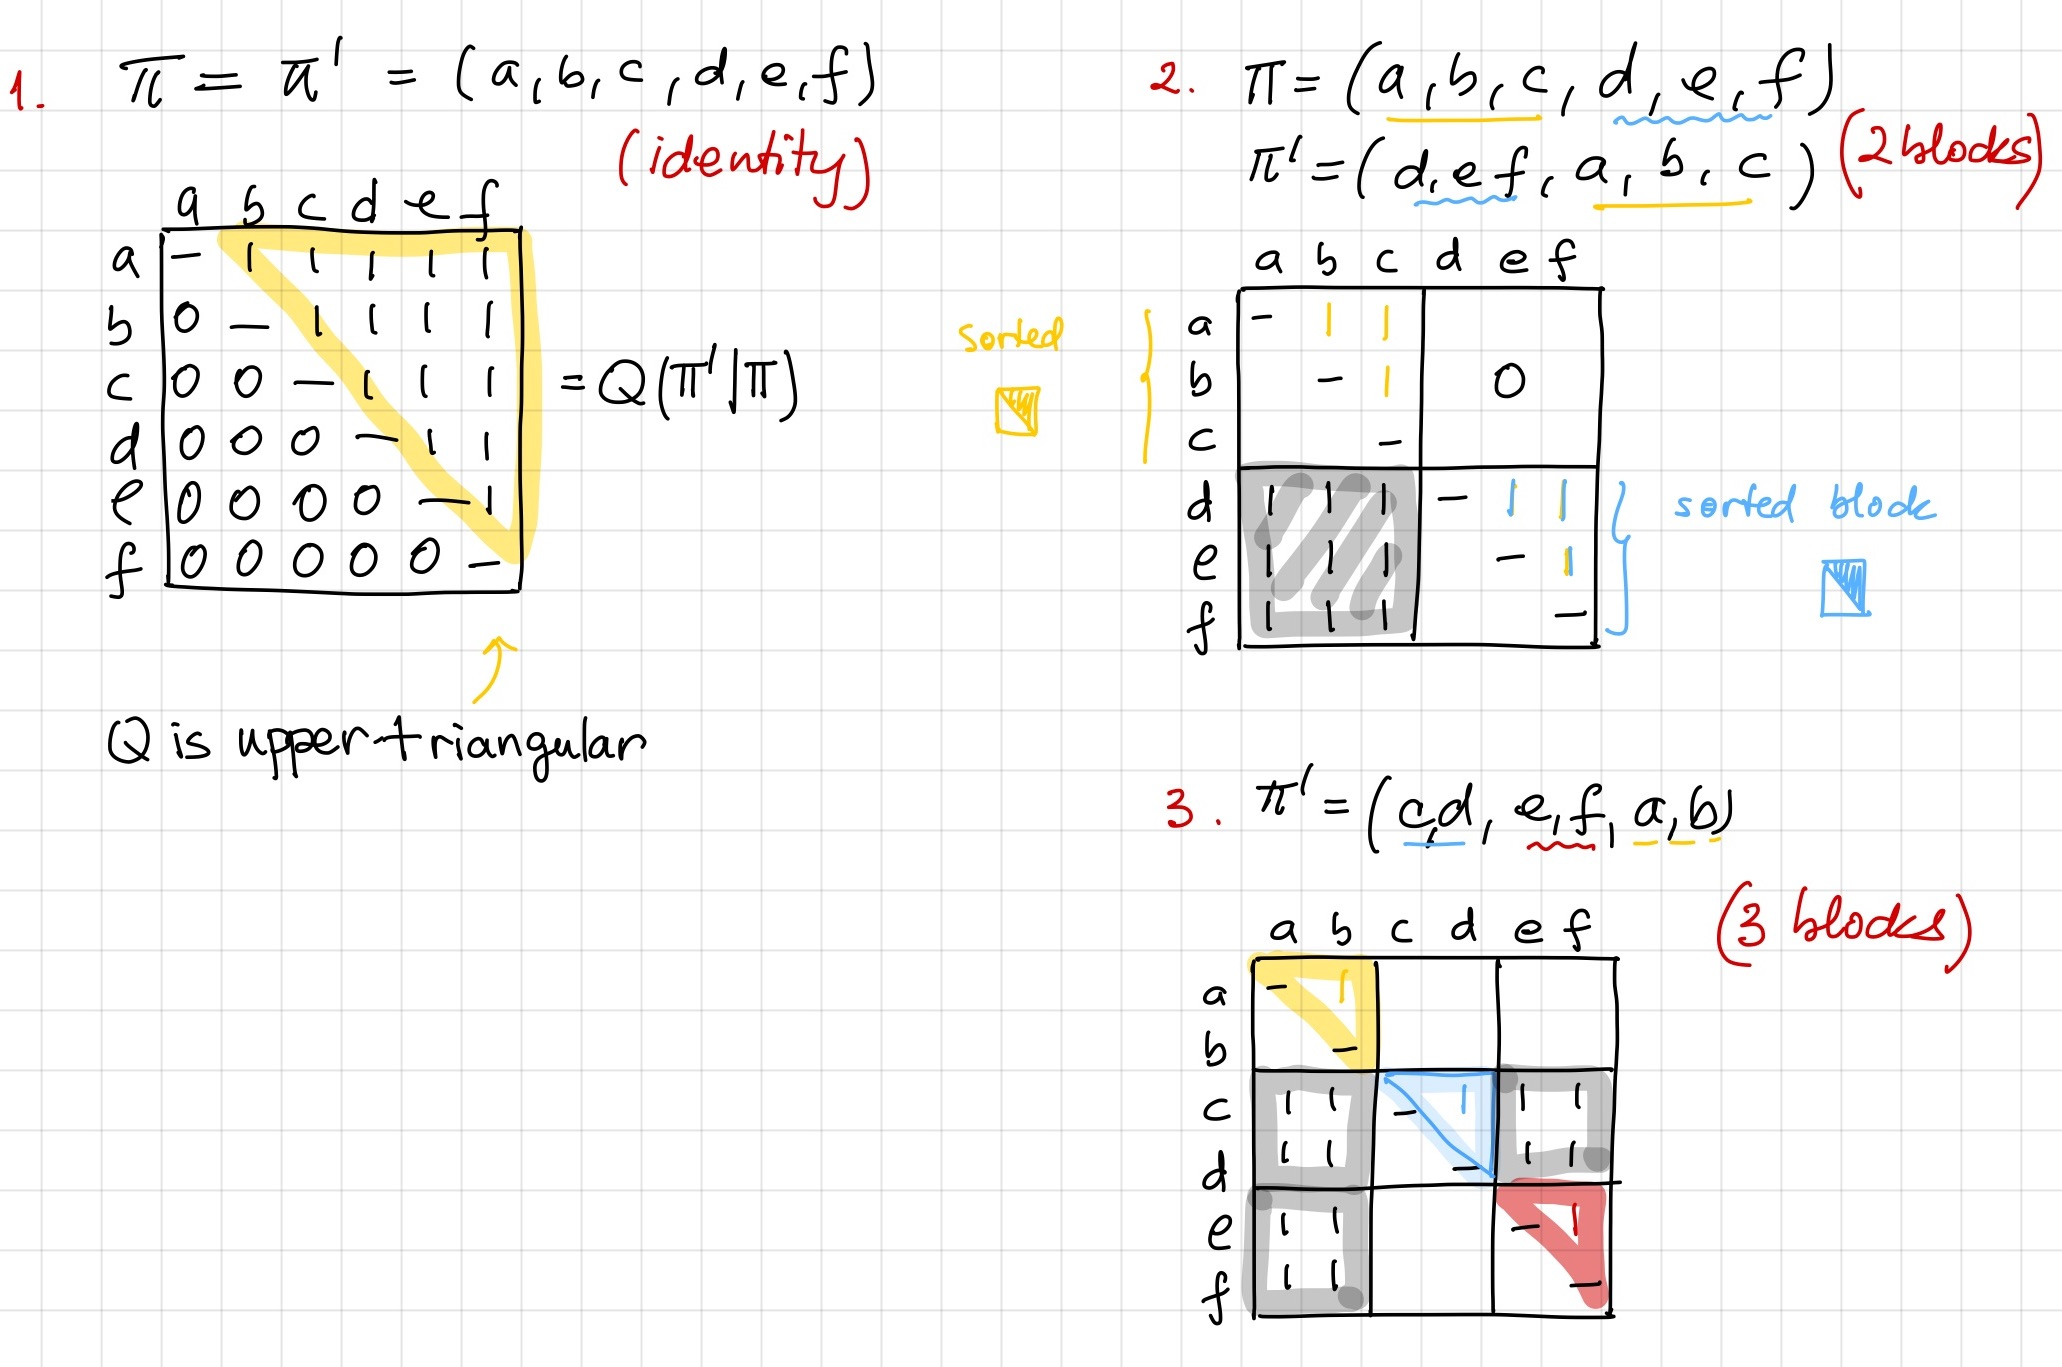
\includegraphics[width=\picwi]{Figs/fig-blocks-Qid-bl.jpg}

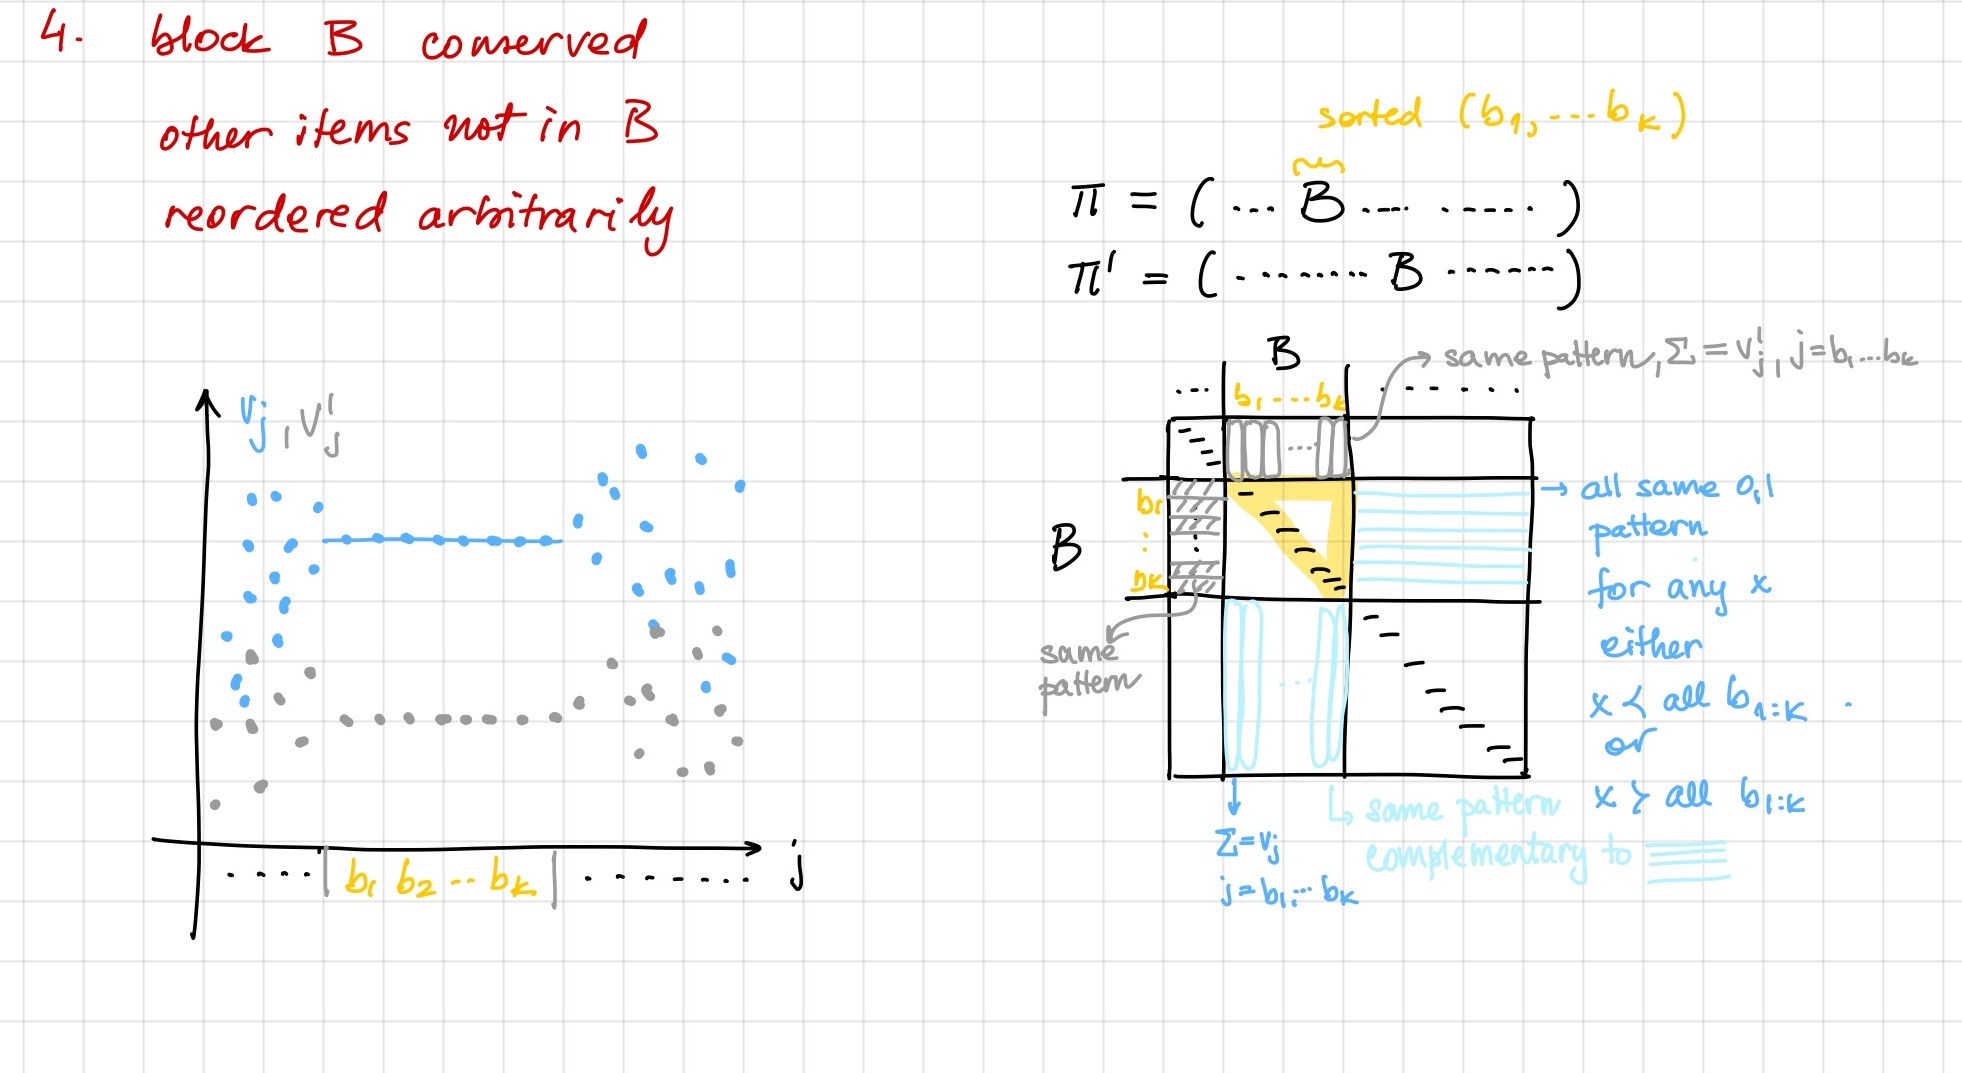
\includegraphics[width=\picwi]{Figs/fig-blocks-QB.jpg}
%
In summary, a block $B$  of size $K$ that stays exactly in the same order in $\pi,\pi'$ can be recognized because $K$ consecutive columns in $Q(\pi'|\pi)$ have the same $v_j$ and $v'_j$. If some elements $x$ from outside $B$ are inserted between elements of $B$ (or, conversely, some $y\in B$ is moved elsewhere) we observe a deviation up or down in the respective column, with a value $K_1, K-K_1 < K$. This is regardless of how $\pi'$ reorders $\X_0\setminus B$, the other elements of $\pi$.

\section{Block detection}
\label{sec:alg-block}
When the above are only approximatively true, we expect that
$v_j,v'_j$ are only approximatively constant over $B$, with a small
number of values off by less than $K$ (for the inserts/deletes from
$B$).

Hence, we are looking for regions where $v,v'$ are approximately
constant over a range $1:n_0$. The following algorithm (sketch) can
do this.
\begin{algorithm}{Algorithm {\sc Find-Blocks}}
\begin{algorithmic}[1]
  \State {\bf Input} $L$ length of block, $p$ outlier fraction (e.g. $p=0.05$)
  \State {compute $v_j,v'_j$ for $j=1:n$}
  \For{$j=L:n$}
  \State {$m_j=\algrobme(v_{j-L+1:j},p)$}
  \State {$m'_j=\algrobme(v'_{j-L+1:j},p)$}
  \State {$s_j=\algrobsd(v_{j-L+1:j},p)$}
  \State {$s'_j=\algrobsd(v'_{j-L+1:j},p)$}
  \EndFor
  \State [Plot $v_j,v'_j$ vs $j$ -- see figure above]
  \State {Find in the plot above regions of length $L$ or larger where $m_j,m'_j\approx$ constant, and $s_j,s'_j\ll L$}
  \State {Merge overlapping blocks if their average $m_j$ values are similar, or leave them separate otherwise}
\end{algorithmic}
\end{algorithm}
%
The $L$ value should be $L\leq K/2$ since for the first $1:L-1$ of a block the means may not be constant and the variances may be larger.  Intuitively, if one expects blocks of length $K=200\ldots 1000$, then $L=100$ would be a reasonable choice.

\section{Using Algorithm {\sc Find-Blocks}}

\paragraph{Lists $\pi,\pi'$  don't have the same elements}
If a block $B$ is conserved between $\pi$ and $\pi'$, then it must contain only items common to the two lists; $B\subset \pi\cap \pi'$. However, it's possible that there are larger sets $B_0,B_0'$ with  $B\subset B_0\subset \pi$, and   $B\subset B_0'\subset \pi'$.

So, the {\sc Find-Blocks} algorithm can be used as follows.

\begin{algorithm}{}
\begin{algorithmic}[1]
  \State Find set $\X_0=\pi\cap \pi'$ (finite)
  \State Guess $K$ length of block, $p$ outlier fraction, set $L=K/2$
  \State Blocks $\{B,\ldots\}=\text{\sc Find-Blocks}(\pi_{|\X_0},\pi'_{|\X_0},L,p)$
  \For{$B$ block}
  \State Find $B$ in $\pi$; if among the items in $B$ item $a\not\in\pi'$ is found, add $a$ to $B_0$. 
  \State Find $B$ in $\pi'$; if among the items in $B$ item $a'\not\in\pi$ is found, add $a'$ to $B_0'$. 
  \EndFor
\end{algorithmic}
\end{algorithm}

\paragraph{Are the top-100 items in $\pi$ a block?}
One can also take a block of interest, such as the top-$K$ of $\pi$
and check if it is preserved in $\pi'$. Let's call this block $B$. For
this, we would compute $v_j,v'_j$ for $j=1:K$, then
$m_j=\algrobme(v_{1:K},p)$, $m'_j=\algrobme(v'_{1:K},p)$,
$s_j=\algrobsd(v_{1:K},p)$, $s'_j=\algrobsd(v'_{1:K},p)$.

\paragraph{Computing $v_j,\,v'_j$  without constructing $Q$, or by using only the lower triangle}  This follows from their definitions (above \eqref{eq:vj}). 


\end{document}
